\documentclass[preprint,12pt,a4paper]{elsarticle}

\usepackage{amssymb}
\usepackage{float}
\usepackage{listings}
\PassOptionsToPackage{hyphens}{url}
\usepackage{hyperref}
\usepackage{xcolor}
\usepackage{lineno}
\setlength{\parindent}{0pt}
\emergencystretch=3em
\sloppy
\lstdefinestyle{mystyle}{
    basicstyle        = \ttfamily\footnotesize,
    breakatwhitespace = false,
    breaklines        = true,
    captionpos        = b,
    keepspaces        = true,
    numbersep         = 5pt,
    showspaces        = false,
    showstringspaces  = false,
    showtabs          = false,
    keywordstyle      = \color{blue},
    stringstyle       = \color{green},
    commentstyle      = \color{red}\ttfamily
}
\lstset{style=mystyle}

\restylefloat{table}
\journal{SoftwareX}

% ---------------------------------------------------------------------------
% TODO(authors) -- resolve before resubmission: \datarepo must resolve publicly.
% The instances, raw results and verification tables now live in this repository
% under benchmarks/, so the link below is the article repository itself; it has
% to be public (or archived with a DOI) before resubmission, since reviewers 2
% and 3 both flagged the previous, unreachable data link.
% ---------------------------------------------------------------------------
\newcommand{\datarepo}{https://github.com/lpawela/bruteforce-text}
\newcommand{\datareponame}{\texttt{lpawela/bruteforce-text}}

\newcommand{\cudameas}{12.4}

\begin{document}

\begin{frontmatter}

\title{Omnisolver: An extensible interface to Ising spin--glass and QUBO
solvers --- a numerically stabilized, distributed GPU exhaustive-search plugin}

\author[1]{Konrad Ja\l{}owiecki}
\author[2,3]{Jakub Paw{\l}owski}
\author[1,2]{Bart{\l}omiej Gardas}
\author[1,2]{{\L}ukasz Pawela\corref{cor1}}
\ead{lpawela@iitis.pl}

\address[1]{Institute of Theoretical and Applied Informatics, Polish Academy
of Sciences, Ba{\l}tycka 5, 44-100 Gliwice, Poland}

\address[2]{Quantumz.io Sp. z o. o., Pu{\l}awska 12/3, 02-566 Warsaw, Poland}

\address[3]{Institute of Theoretical Physics, Faculty of Fundamental Problems
of Technology, Wroc{\l}aw University of Science and Technology,
50-370 Wroc{\l}aw, Poland}

\begin{abstract}
This software update matures \texttt{omnisolver-bruteforce}, the exhaustive-search
plugin of Omnisolver~\cite{jalowiecki2021omnisolver}, into a released and
API-stable exhaustive-search reference backend for QUBO and Ising
instances on CUDA-enabled GPUs. Throughout, $N$ denotes the number of binary
variables of an instance (equivalently, the number of Ising spins), so that
exhaustive search enumerates all $2^{N}$ configurations. The plugin itself,
together with a preliminary multi-GPU benchmark, was already announced in the
original publication; the present update contributes a released Ray-based
distributed sampler that splits the search into $2^{k}$ fixed-variable
subproblems, dispatches them across multiple GPUs and hosts and merges the
partial results on a controller; numerical stabilization of the fast
\texttt{float32} ground-state path through compensated incremental updates,
periodic from-scratch energy re-anchoring and best-buffer refresh, enabled
automatically for per-kernel subproblems of at least $40$ variables and leaving
the public sampler API unchanged; and 64-bit-safe enumeration bookkeeping that
lifts the reachable problem size beyond the original single-GPU regime. On dense
random Ising instances we report cross-validated exhaustive-search minima up to $N=60$ on
$8\times$ NVIDIA H100 (96\,GB) GPUs, reaching $\approx\!3.15$ days at $N=60$, in
agreement with the empirical $t_{N+1}=2\,t_N$ doubling rule to within $0.3\%$.
Measured against the single-GPU sampler on identical instances, the distributed
sampler crosses over between $N=40$ and $N=42$, attains $93\%$ parallel
efficiency at $N=48$ and saturates at the ideal $8\times$ speedup from
$N\!\gtrsim\!52$; a dedicated sweep over every tested power-of-two GPU count and
realizable node layout gives
$98.2\%$ efficiency on eight GPUs, weak scaling flat to within $0.2\%$, and no measurable
change in the reported solve-phase wall-clock time from crossing a node boundary at constant
computational load. In a
separate twenty-instance,
four-family comparison, both discrete simulated bifurcation and simulated annealing recover
the same exhaustive-search minimum in every case under their stated method-specific budgets.
On a planted Wishart family with tunable ruggedness, by contrast, the same
simulated-bifurcation heuristic misses the certified optimum on $39$ of $40$ instances in the
two most rugged settings while certification takes seconds per instance and matches the
analytic planted optimum to $4\times10^{-15}$ --- the regime a certifying backend exists for.
\end{abstract}

\begin{keyword}
QUBO \sep Ising \sep spin glass \sep exhaustive search \sep GPU \sep
parallel efficiency \sep Omnisolver plugin \sep software update
\end{keyword}

\end{frontmatter}

\section*{Refers to}
K.~Ja\l{}owiecki, {\L}.~Pawela, ``Omnisolver: An extensible interface to Ising
spin--glass and QUBO solvers,'' \emph{SoftwareX} \textbf{24}, 101559 (2023).
DOI: \url{https://doi.org/10.1016/j.softx.2023.101559}.

\section*{Metadata}
\label{metadata}

% TODO(authors): C1/C2 -- the repository at tag 0.0.5 still contains no LICENSE
% file (GitHub license endpoint returns 404, pyproject.toml declares no license,
% PyPI shows no license classifier), so C3 below is not yet backed by the code.
% Reviewer 3 checked this.  Add LICENSE (Apache-2.0), the license field and
% classifier in pyproject.toml, `include LICENSE` in MANIFEST.in and per-file
% license headers, cut release 0.0.6 and bump C1/C2/S1/S2 accordingly.
% TODO(authors): C7 -- the linked documentation redirects to version 0.0.3, has
% no content about this plugin and contains dead links; the plugin's own
% mkdocs.yml references docs/userguide.md and docs/plugins.md, which do not
% exist, so its build is broken.  Either publish the plugin documentation and
% point C7/S6 at it, or point C7 at a page that is actually useful.
\begin{table}[H]
\setlength{\tabcolsep}{4pt}
\begin{tabular}{|l|p{5.6cm}|p{6.4cm}|}
\hline
\textbf{Nr.} & \textbf{Code metadata description} & \textbf{Value} \\
\hline
C1 & Current code version & 0.0.5 \\
\hline
C2 & Permanent link to code/repository used for this code version &
\url{https://github.com/euro-hpc-pl/omnisolver-bruteforce/releases/tag/0.0.5} \\
\hline
C3 & Legal Code License & Apache License 2.0 \\
\hline
C4 & Code versioning system used & git \\
\hline
C5 & Software code languages, tools, and services used & Python, C++, Cython,
CUDA, Ray \\
\hline
C6 & Compilation requirements, operating environments \& dependencies & Linux
(x86-64) with a CUDA-capable NVIDIA GPU; CUDA Toolkit 12.4 and 12.5, both built
and tested in continuous integration; the measurements reported here were
obtained with \cudameas, \texttt{Python >= 3.10}, \texttt{omnisolver >= 0.0.4},
\texttt{dimod ~= 0.12}, \texttt{numba ~= 0.58}, \texttt{numpy ~= 2.0};
\texttt{ray >= 2.9} is additionally required by the distributed sampler \\
\hline
C7 & Link to developer documentation/manual &
\url{https://euro-hpc-pl.github.io/omnisolver/} \\
\hline
C8 & Support email for questions & \verb|lpawela@iitis.pl| \\
\hline
\end{tabular}
\caption{Code metadata}
\label{codeMetadata}
\end{table}

\begin{table}[H]
\setlength{\tabcolsep}{4pt}
\begin{tabular}{|l|p{5.6cm}|p{6.4cm}|}
\hline
\textbf{Nr.} & \textbf{(Executable) software metadata description} &
\textbf{Value} \\
\hline
S1 & Current software version & 0.0.5 \\
\hline
S2 & Permanent link to executables of this version &
\url{https://pypi.org/project/omnisolver-bruteforce/0.0.5/}; the distribution is
a source archive, so the CUDA extension is compiled at installation time against
the CUDA Toolkit available on the target machine \\
\hline
S3 & Legal Software License & Apache License 2.0 \\
\hline
S4 & Computing platforms/Operating Systems & Linux (x86-64) with a CUDA-capable
NVIDIA GPU; the reported measurements were performed on NVIDIA H100 96\,GB
(compute capability \texttt{sm\_90}) \\
\hline
S5 & Installation requirements \& dependencies & CUDA Toolkit 12.4 or 12.5
(both exercised in continuous integration; measurements: \cudameas), \texttt{Python >= 3.10},
\texttt{omnisolver >= 0.0.4}, \texttt{dimod}, \texttt{numba}, \texttt{numpy};
\texttt{ray >= 2.9} for the distributed sampler; at build time additionally
\texttt{cython} and \texttt{setuptools-cuda} \\
\hline
S6 & Link to user manual & \url{https://euro-hpc-pl.github.io/omnisolver/} \\
\hline
S7 & Support email for questions & \verb|lpawela@iitis.pl| \\
\hline
\end{tabular}
\caption{Software metadata}
\label{softwareMetadata}
\end{table}

\linenumbers

\section{Description of the software update}
\label{sec:description}

Omnisolver~\cite{jalowiecki2021omnisolver} is a plugin-based framework that
exposes a uniform Python and command-line interface to QUBO/Ising solvers,
integrated with \texttt{dimod}. A solver is contributed as an independent
package that registers itself through an entry point and ships a small
specification file, from which the framework derives the command-line interface
and the input/output handling; solvers can therefore be interchanged without
touching the surrounding workflow. The original publication established the
framework together with its first plugins, among them a parallel-tempering
sampler and the exhaustive-search plugin discussed here. This update concerns
the latter, \texttt{omnisolver-bruteforce}: it turns the plugin into a released,
API-stable certification backend, contributes a distributed multi-GPU sampler
built on Ray~\cite{DBLP:journals/corr/abs-1712-05889}, and stabilizes the
numerical behavior of its fast ground-state path.

Throughout this paper, $N$ denotes the number of binary variables of an instance
(equivalently, the number of Ising spins), so that exhaustive search enumerates
all $2^{N}$ configurations. The remaining quantities used below are the
parameters exposed by the plugin's samplers: \texttt{num\_states} is the number
of lowest-energy states to be returned, \texttt{num\_fixed\_vars}\,$=k$ is the
number of variables whose values are frozen in order to define independent
subproblems in the distributed sampler, and \texttt{suffix\_size} is the number
of variables forming the enumeration suffix, i.e.\ $2^{\texttt{suffix\_size}}$
configurations are resident in the GPU working set at a time and the search
sweeps $2^{N-\texttt{suffix\_size}}$ such chunks. The parameters
\texttt{grid\_size} and \texttt{block\_size} control the CUDA launch geometry,
while \texttt{num\_steps\_per\_kernel} and \texttt{partial\_diff\_buffer\_depth}
set the number of chunks processed per kernel launch and the depth of the
incremental-energy buffers, respectively.

\paragraph{Purpose of an exhaustive solver in Omnisolver}
An exhaustive backend provides reference solutions by evaluating every configuration. With
exactly representable coefficients and arithmetic this establishes a global optimum; on the
plugin's fast floating-point path the ordering is necessarily numerical. Throughout this paper,
``certified'' therefore means the minimum selected by complete enumeration and independently
cross-validated as described below, rather than a formal interval- or exact-arithmetic proof for
arbitrary real-valued coefficients. Such reference answers are essential for
benchmarking approximate or heuristic methods, for verifying NISQ-oriented
workflows~\cite{preskill2018quantum}, and for assessing claims of quantum
runtime advantage. In recent years, the latter point has become especially
critical in the community, with many studies relying on metrics that
explicitly depend on the ground-state energy, such as the \emph{optimality gap}.
For example, in recent comparative studies of runtime
advantage~\cite{tuziemski2026limits} and of the quantum-classical scaling
gap~\cite{pawlowski2025closing}, quantum resources were benchmarked against the
Simulated Bifurcation Machine
(SBM)~\cite{goto2016bifurcation,goto2019combinatorial,goto2021high,pawlowski2026sbqa},
the current state-of-the-art classical heuristic for dense QUBO/Ising problems.
Such results rely on high-confidence global reference minima on representative
instances, which is precisely the role of an exhaustive GPU solver. A concrete
case in which the heuristic's answer is wrong and only enumeration can tell is
reported below.

\paragraph{Architecture}
The plugin exposes two sampler classes: \texttt{BruteforceGPUSampler}
(single-node, single-GPU) and \texttt{DistributedBruteforceGPUSampler}
(multi-GPU/multi-node via Ray). The distributed sampler fixes
\texttt{num\_fixed\_vars}\,$=k$ variables and enumerates all $2^{k}$ fixed
assignments; each assignment becomes an independent subproblem with $N-k$
unfixed variables, dispatched as a Ray task and solved by the GPU kernel on a
worker. Partial solutions are collected and merged on the controller node. Both
samplers accept SPIN and BINARY models: a SPIN model is converted to its BINARY
equivalent, solved as a QUBO and converted back, so the QUBO and Ising code
paths coincide up to a host-side transformation performed outside the measured
region. As a practical guideline, the single-GPU sampler remains the right
choice as long as a single device has sufficient memory and the expected
wall-clock time is acceptable; beyond that point the distributed sampler
amortizes the work by powers of two in the number of workers. On our hardware it
crosses the break-even region between $N=40$ and $N=42$ (see
Fig.~\ref{fig:runtimes} and Table~\ref{tab:efficiency}), and from
$N\!\gtrsim\!52$ it attains the full $\approx\!8\times$ speedup expected from
the 8-GPU pool, once Ray-scheduling and kernel-launch overheads are amortized
over the per-subproblem computation. Performance-critical kernels are
implemented in CUDA/C++ and exposed to Python via Cython; the
\texttt{num\_states=1} fast path operates in \texttt{float32}, halving the size of
the resident energy buffers, with the stabilization mechanisms described below
compensating for the resulting roundoff. Note that on the hardware measured here
single precision buys working-set size rather than speed: the timing suggests that the
enumeration is limited by memory traffic and integer bookkeeping rather than by floating-point throughput,
and double precision costs only a few percent (see below).

\paragraph{Relation to the original publication and to the predecessor solver}
The exhaustive-search plugin is not new, and we state its provenance
explicitly. The original Omnisolver
publication~\cite{jalowiecki2021omnisolver} already lists
\texttt{omnisolver-bruteforce} among the available plugins, notes that it can be
accelerated on CUDA-enabled GPUs, describes it as usable for instances of up to
about $50$ variables, and reports a preliminary benchmark of the GPU sampler on
$1$, $2$, $4$ and $8$ NVIDIA A100 GPUs. Its computational core goes back further
still, to the stand-alone single-GPU solver of~\cite{jalowiecki2021brute}: on
instances that fit a single device the present kernel is API-compatible with
that solver and reproduces its per-state throughput within measurement noise, so
this update does not re-benchmark the single-device axis but inherits its
performance envelope. What the update contributes is therefore not the existence
of a GPU-accelerated or multi-GPU exhaustive search, but its maturation into a
dependable certification backend, as detailed next.

\paragraph{Update contributions}
\begin{itemize}
    \item \textbf{Released, API-stable distributed sampler}: the multi-GPU code
    path is now a documented, versioned public class
    (\texttt{DistributedBruteforceGPUSampler}, tagged \texttt{0.0.5} and
    published on PyPI) rather than the unreleased code behind the preliminary
    benchmark of~\cite{jalowiecki2021omnisolver}, and it returns a
    \texttt{dimod.SampleSet} carrying runtime metadata through the same plugin
    and CLI mechanism as any other Omnisolver sampler.
    \item \textbf{Stabilized fast ground-state path}: compensated incremental
    updates, periodic from-scratch energy re-anchoring and a final refresh of the
    best-state buffer mitigate the \texttt{float32} drift previously observed
    in the \texttt{num\_states=1} mode. Stabilization is enabled automatically
    whenever the size seen by the kernel is at least $40$ variables, that is for
    $N-k \geq 40$ in distributed runs; the public API is unchanged.
    \item \textbf{Hardening for large-$N$ enumeration}: 64-bit-safe bit
    operations and kernel-step bookkeeping make the enumeration correct for
    configuration sizes well beyond the original single-GPU regime.
    \item \textbf{Certification reach and scaling evidence}: measurements are
    extended from the $N\approx 50$ of~\cite{jalowiecki2021omnisolver} to
    $N=60$, i.e.\ by three orders of magnitude in enumerated configurations, and
    are accompanied by an explicit strong-scaling efficiency analysis
    (Table~\ref{tab:efficiency}) and by an end-to-end verification of the
    returned optima.
    \item \textbf{Extended validation}: GPU tests cross-check energies against
    from-scratch exact recomputation and against \texttt{dimod.ExactSolver} on
    instances small enough for CPU enumeration; at benchmark scale, the returned
    configurations are additionally re-verified outside the plugin by a
    from-scratch \texttt{float64} energy recomputation and cross-checked against
    an independent heuristic solver.
\end{itemize}

\paragraph{Performance}
Figure~\ref{fig:runtimes} reports wall-clock solve times of both sampler modes on
all-to-all random Ising instances with $J_{ij},h_i\sim \mathcal{U}[-1,1]$ i.i.d.,
generated by the benchmark script \texttt{benchmarks/bf.py} of the article repository
(one archived instance per size; these shipped instance files, rather than an unrecoverable
legacy RNG state, define the benchmark; see Sec.~\ref{sec:reproduction}) and measured on a local
in-house cluster of $8\times$ NVIDIA H100 (96\,GB) GPUs (two nodes, 4 GPUs per
node, interconnected by standard Ethernet). The single-GPU sampler was run on one
of the same H100s and the distributed sampler on all eight, with $k=3$ so that
the $2^{3}=8$ subproblems map one-to-one onto the available GPUs; both modes used
\texttt{suffix\_size}\,$=23$ and \texttt{num\_states}\,$=1$.

Reported times measure the solve phase only. For the single-GPU sampler the timer
brackets the CUDA search itself, excluding host-side assembly of the QUBO matrix
and decoding of the returned configurations; for the distributed sampler it
brackets subproblem dispatch and the collection of all partial results on the
controller, excluding the final merge of those partial results, which is
discussed separately below. Both exclusions are polynomial in $N$ and negligible
at the sizes reported here, but they matter for the extrapolations discussed
further on.

The $O(2^N)$ doubling per added spin is the dominant feature of both curves: the
measured single-GPU times grow by a factor of $2.001$--$2.002$ per added variable
over the whole range $N=42,\dots,54$. The one departure is the first step,
$N=40\to42$, which grows by $2.993$ rather than by $4$; this is an artifact of the
first measurement in a process paying the one-off creation of the CUDA context.
Re-measuring $N=40$ after a warm-up gives $2.11$\,s instead of $2.74$\,s, and
$4\times 2.11=8.4$\,s then agrees with the measured $8.20$\,s at $N=42$. The
$\approx\!0.6$\,s involved is invisible at every larger size and affects no
conclusion, but it does inflate the $N=40$ entries of Fig.~\ref{fig:runtimes} and
Table~\ref{tab:efficiency}. The distributed curve flattens out for $N \lesssim 44$,
because timings are dominated there by kernel-launch and Ray-scheduling overhead,
and settles onto the same asymptotic slope ($1.998$--$2.003$ per variable) from
$N=52$ onward. The largest measured size, $N=60$ in the distributed mode, takes
$\approx\!272{,}300$ s ($\approx 3.15$ days), within $0.3\%$ of the
doubling-rule extrapolation from $N=58$ ($2^{2}\!\times\!67{,}900 \approx
271{,}600$ s); this confirms that the distributed curve is in its asymptotic
$t_{N+1}=2\,t_N$ regime at the upper end of the measured range. We use the same rule to project
the single-GPU sampler (measured
up to $N=54$) to $N=60$ along the dashed extension in Fig.~\ref{fig:runtimes}:
the projected single-GPU wall-clock at $N=60$ is $\approx\!2.17\times 10^{6}$ s
($\approx\!25$ days), about $8.0\times$ the measured 8-GPU time at the same size
and consistent with linear strong scaling. The same rule places $N=64$ at
$\approx\!50$ days on the 8-GPU pool. Constant-factor deviations from exact
doubling (kernel-launch overhead, host/device transfer, Ray scheduling) may shift
the absolute numbers by a few percent on nearby sizes or different stacks without changing the
asymptotic scaling.

\paragraph{Strong scaling and parallel efficiency}
Because both samplers were run on the same instances, the two curves of
Fig.~\ref{fig:runtimes} can be paired size by size into an explicit
strong-scaling measurement, reported in Table~\ref{tab:efficiency} in terms of
the speedup $S=t_1/t_8$ and the parallel efficiency $E=S/8$. Below the crossover
the decomposition is dominated by fixed overheads: at $N=40$ the eight-way split
is in fact $2.1\times$ \emph{slower} than a single GPU, which is why the
single-GPU sampler remains the appropriate choice below the crossover.
Efficiency then rises steeply, from $43\%$ at $N=44$ through $75\%$ at $N=46$ and
$93\%$ at $N=48$, and saturates at the ideal value from $N=52$ on, where the
per-subproblem computation dwarfs dispatch and launch overheads. The marginal
excess over unity at $N=54$ ($E=100.1\%$) is within the run-to-run variability of
these single-run timings and should be read as ideal scaling rather than as
superlinear speedup. This behavior is the expected signature of an
embarrassingly parallel decomposition whose fixed cost per subproblem is
independent of $N$: the eight-GPU pool becomes fully efficient exactly once
$2^{N-k}$-configuration subproblems are large enough to amortize that cost.

\begin{table}[H]
\centering
\begin{tabular}{|r|r|r|r|r|}
\hline
$N$ & $t_1$ [s] & $t_8$ [s] & $S=t_1/t_8$ & $E=S/8$ \\
\hline
40 & 2.74      & 5.68     & 0.48 & 6\% \\
42 & 8.20      & 6.52     & 1.26 & 16\% \\
44 & 32.83     & 9.48     & 3.46 & 43\% \\
46 & 131.54    & 21.90    & 6.01 & 75\% \\
48 & 527.07    & 71.17    & 7.41 & 93\% \\
50 & 2112.29   & 268.90   & 7.86 & 98\% \\
52 & 8458.17   & 1060.68  & 7.97 & 99.7\% \\
54 & 33912.27  & 4235.25  & 8.01 & 100.1\% \\
\hline
\end{tabular}
\caption{Strong-scaling speedup and parallel efficiency of the distributed
sampler ($t_8$, $8\times$ H100, $k=3$) relative to the single-GPU sampler
($t_1$, one H100 of the same cluster) on identical instances; the timings are the
measured points of Fig.~\ref{fig:runtimes}. Efficiency stays below unity for
$N \lesssim 46$ because kernel-launch and Ray-scheduling overheads are not yet
amortized, exceeds $90\%$ from $N=48$ and saturates at the ideal value from
$N=52$ on. The value at $N=54$ marginally exceeds unity; repeating the measurements of
Table~\ref{tab:scaling} showed two-node timings such as $t_8$ reproducing only to within
$\approx\!0.5\%$, which covers the $0.1\%$ excess. The $N=40$ row overstates the efficiency:
being the first measurement of its sweep, $t_1$ there includes the one-off CUDA
context creation discussed in the text, and drops to $2.11$\,s when re-measured
after a warm-up.}
\label{tab:efficiency}
\end{table}

\paragraph{Scaling with the GPU count and with the node layout}
Table~\ref{tab:efficiency} varies the problem size at a fixed eight GPUs. The complementary
measurement---fixing the problem and varying the machine---is reported in
Table~\ref{tab:scaling}, and it also separates \emph{how many} GPUs are used from \emph{how
they are distributed over nodes}, which is the question the two-node geometry of our cluster
allows us to probe. Since Ray cannot rearrange a running cluster, each row was taken on a
cluster started afresh in the corresponding layout, written $\langle$nodes$\rangle\times
\langle$GPUs per node$\rangle$; the sampler detects the layout it is given and records it with
the measurement.

Strong scaling at $N=50$ is close to ideal: $2.00\times$ on two GPUs, $3.99\times$ on four and
$7.86\times$ on eight, i.e.\ a parallel efficiency of $98.2\%$ at the full pool. Two features
are worth singling out. First, the distributed sampler configured with $k=0$ on a single GPU
takes $2113.1$\,s against $2112.9$\,s for the single-GPU sampler on the same instance: at this
size the explicitly separated dispatch and merge phases total $0.032$\,s, while the full
runtimes differ by $0.2$\,s ($0.009\%$). Both are negligible beside the search once the
subproblems are large. Second, comparing $2\times1$ against $1\times2$ and $2\times2$ against $1\times4$
isolates the cost of crossing a node boundary at constant computational load, and that cost is not
resolvable: the two-node configuration is faster by $0.03\%$ in the first pair and by $0.12\%$
in the second. Repeating the entire series on a different day is what establishes the
resolution. Single-node configurations reproduced to within $0.08\%$ across both sweeps
($0.02\%$ in the strong-scaling half), but two-node ones moved by up to $1.5\%$, always in the
same direction: the first run's two-node points were uniformly
the slower ones. We therefore report no measurable node-boundary effect on the reported
solve-phase wall-clock time at constant computational load; the observed $1.5\%$ two-node
repeatability is
an empirical resolution scale, not a statistical upper bound on the boundary effect. This
is consistent with the absence of inter-worker communication during the search and localizes
the observed variability only to the two-node/second-host path, not to a particular mechanism.

Weak scaling, in the right-hand half of Table~\ref{tab:scaling}, grows $k$ together with the
device count so that every GPU always enumerates $2^{50}$ configurations. The wall-clock time
stays between $2112.5$\,s and $2116.9$\,s across the whole series, i.e.\ flat to within
$0.2\%$ from one to eight GPUs and from $N=50$ to $N=53$, with the merge contributing
approximately $0.007$\,s throughout. Ideal weak scaling would keep this row constant, and within the
resolution established above it does.

\begin{table}[H]
\setlength{\tabcolsep}{4pt}
\centering
\small
\begin{tabular}{|l|r|rrr|rrr|}
\hline
 &  & \multicolumn{3}{c|}{strong scaling, $N=50$} &
\multicolumn{3}{c|}{weak scaling, $2^{50}$ per GPU} \\
layout & $P$ & $t$ [s] & $S$ & $E$ & $N$ & $t$ [s] & $t/t_1$ \\
\hline
single-GPU sampler & 1 & 2112.9 & --- & --- & 50 & 2112.9 & 1.000 \\
$1\times1$ & 1 & 2113.1 & 1.00 & 100.0\% & 50 & 2113.1 & 1.000 \\
$1\times2$ & 2 & 1056.7 & 2.00 & 100.0\% & 51 & 2112.9 & 1.000 \\
$2\times1$ & 2 & 1056.3 & 2.00 & 100.0\% & 51 & 2112.5 & 1.000 \\
$1\times4$ & 4 & 530.2  & 3.99 & 99.6\%  & 52 & 2116.6 & 1.002 \\
$2\times2$ & 4 & 529.5  & 3.99 & 99.8\%  & 52 & 2114.5 & 1.001 \\
$2\times4$ & 8 & 268.9  & 7.86 & 98.2\%  & 53 & 2116.9 & 1.002 \\
\hline
\end{tabular}
\caption{Strong and weak scaling of the distributed sampler over GPU count and node layout,
on $8\times$ NVIDIA H100 (96\,GB) across two nodes. A layout $n\times m$ means $n$ nodes with
$m$ GPUs each, obtained by masking the visible devices before starting Ray; $P=nm$ is the
total GPU count and $k=\log_2 P$ places one subproblem on each device. Strong scaling solves
the same $N=50$ instance on every layout, with $S=t_1/t_P$ against the single-GPU sampler and
$E=S/P$. Weak scaling grows the size with the device count, $N=50+k$, so that the work per GPU
is constant at $2^{50}$ configurations; $t_1$ is the single-GPU sampler. The pairs
$1\times2$/$2\times1$ and $1\times4$/$2\times2$ hold $P$ fixed and differ only in the number of
node boundaries crossed. The whole series was measured twice, on separate days; the values
quoted are from the second run. Single-node configurations reproduced to within $0.08\%$
between the two runs ($0.02\%$ in the strong-scaling half), and two-node ones to within
$1.5\%$, which is what limits the resolution of
the node-boundary comparison.}
\label{tab:scaling}
\end{table}

The top-level strong- and weak-scaling result files contain the second pass quoted in the table. The first H100
pass is retained in the article repository history at commit \texttt{d965e54}; the percentages
above are recomputed from those two sets of raw timings.

\paragraph{Controller cost and the limits of the decomposition}
The search phase itself involves no inter-worker communication: each of the
$2^{k}$ subproblems is an independent Ray task that fixes its own variables, runs
the CUDA search over the remaining $N-k$ and returns only the requested
\texttt{num\_states} samples. The single point of centralization is the
controller, which retrieves the $2^{k}$ partial sample sets and merges them into
one. Whether that centralization limits the decomposition is a fair question, and part of it can be
answered without a large allocation: the number of subproblems is set by
\texttt{num\_fixed\_vars} and is independent of the number of devices, so the controller can be
driven on a CPU alone with the partial results that workers would have returned.
Table~\ref{tab:controller} reports that measurement for $2^{k}$ subproblems with $k$ up to
$16$, comparing the direct merge --- collect every partial result on the controller and
concatenate once --- with a hierarchical merge performed by a tree of Ray tasks, and both
against the floor set by Ray's task scheduling alone.

It is important to be clear about what this does and does not cover. Running on one machine,
every partial result is local and every task is scheduled by the local raylet, so the numbers
contain merge arithmetic and local scheduling but no inter-node transfer. They are therefore a
lower bound on controller cost at a given $P$, not an estimate of the total: a real allocation
would additionally move result bytes across the fabric and place scheduling load on a shared
head node. Within that bound, three things follow. First, the direct merge grows essentially
linearly in the number of subproblems, as expected for sequential concatenation: a log--log fit
to the measured points gives $O(P^{0.99})$ over four decades, rather than the logarithmic
scaling that a tree reduction would exhibit. Second, merge arithmetic is not the limiting local component: at
$2^{16}=65{,}536$ subproblems concatenation accounts for $2.1$\,s of the $7.4$\,s direct-merge
measurement. Third, dispatching and collecting $2^{16}$ \emph{empty} tasks already costs
$5.4$\,s. This is a scheduling floor only; a real payload-bearing task additionally pays for
serialization, delivery and materialization.

Ray can return small values inline with the task-completion reply, avoiding a separate pull
through the distributed object store. Inline delivery does not eliminate network transfer: the
bytes still travel in the completion message. Consequently neither the empty-task floor nor the
single-machine merge measurements quantify the end-to-end cost of a node boundary, and we do
not infer one from Table~\ref{tab:controller}. The reproduction package includes
\texttt{benchmarks/exp\_boundary\_cost.py}, which compares matched tasks from submission through
\texttt{ray.get}: both receive the same serialized request and construct the same
\texttt{SampleSet}, but only one returns it. Local, remote and mixed placements are measured,
and every repetition is retained. This ordinary task-return path includes whichever delivery
mechanism Ray selects; it measures the aggregate effect rather than separately identifying
serialization, transport, storage or materialization costs. Even on two nodes it cannot
establish whether a head node or fabric saturates when thousands of workers report
simultaneously.

For batches of sixteen tasks, the paired remote-minus-local effect of returning the payload
rather than discarding it was $196.45$\,$\mu$s per task for a $50{,}165$-byte result and
$4.404$\,ms per task for a $496{,}575$-byte result. Across five repetitions the corresponding
ranges were $192.63$--$220.02$\,$\mu$s and $4.340$--$4.426$\,ms per task. The $1{,}061$-byte
case was dominated by scheduling variability, and the larger-batch measurements were noisier,
so we retain all raw observations and do not fit a bandwidth model. These are aggregate
ordinary Ray return-path effects on this two-node cluster, not isolated network-transfer
times. The production record is
\path{benchmarks/results/boundary_cost/2x1_production_20260816T122920_076038Z.json}.

This unresolved many-node centralization is itself the argument for the hierarchical merge: reducing
through a tree leaves the controller receiving a single object instead of $P$, reducing both
its ingress count and its memory pressure rather than merely accelerating concatenation.

The hierarchical merge first overtakes the direct one at $P=64$, where its
logarithmic depth starts to beat the linear cost of fetching every partial result,
and beyond that it also bounds the memory the controller needs. Both strategies are
available in the released sampler. Its conservative automatic policy uses the direct path
through $P=64$ and switches to the hierarchy above it ($P\geq128$); through $P=64$ the two
differ by at most $1.9$\,ms. What remains
true is that at fixed $N$ incrementing $k$ halves the work per subproblem while
doubling the number of results to combine, so a break-even point in $k$ exists ---
the measurement quantifies the growing controller term and locates the merge-strategy
crossover, but the full solver's search-versus-controller break-even on a large allocation
remains unmeasured.

\begin{table}[H]
\centering
\small
\begin{tabular}{|r|r|r|r|r|}
\hline
$P=2^{k}$ & concatenation & direct merge & hierarchical merge & Ray floor \\
\hline
$2^{8}$  & 0.008 & 0.026 & 0.014 & 0.039 \\
$2^{10}$ & 0.030 & 0.111 & 0.047 & 0.084 \\
$2^{12}$ & 0.124 & 0.472 & 0.189 & 0.300 \\
$2^{14}$ & 0.523 & 1.906 & 0.893 & 1.325 \\
$2^{15}$ & 1.039 & 3.849 & 1.860 & 2.605 \\
$2^{16}$ & 2.050 & 7.408 & 3.811 & 5.397 \\
\hline
\end{tabular}
\caption{Controller-side cost, in seconds, of combining the partial results of $P$
subproblems, measured on a CPU with \texttt{num\_states}$\,=1$ and $N=60$ and therefore
without requiring $P$ GPUs. \emph{Concatenation}: the merge arithmetic alone, with the partial
results already in the controller's memory. \emph{Direct merge}: fetching all $P$ partial
results and concatenating them once. \emph{Hierarchical merge}: the same reduction performed by
a tree of Ray tasks combining eight results at a time. \emph{Ray floor}: dispatching and
collecting $P$ empty tasks, which no strategy that dispatches $P$ Ray tasks can beat. All four columns are
measured on a single machine and therefore exclude network transfer between nodes; they bound
the local component of the controller cost from below rather than estimating its total. Medians of five
repetitions after a warm-up, from one sweep over $k=3,\dots,16$; the rows for $k<8$ are omitted
for compactness. A separate sweep put the crossover between the two merge strategies at the
same $P=64$.}
\label{tab:controller}
\end{table}

\paragraph{Scaling outlook on larger allocations}
Since the search phase is embarrassingly parallel, the size reachable on a larger
allocation follows from the measured 8-GPU baseline by simple proportionality,
for as long as the controller cost discussed above stays subdominant. As a
back-of-the-envelope projection, scaling to $2^{14}=16{,}384$ GPUs --- a
partition size within reach of current leadership-class systems --- with the
natural choice $k=14$ placing one subproblem per worker would reduce $N=60$ from
$\approx\!3.15$ days to $\approx\!2.2$ min, and the projected $N=64$ time from
$\approx\!50$ days to $\approx\!35$ min. Under a one-month wall-clock budget on
the same allocation, the doubling rule places the limit for certifiable
exhaustive search at $N \lesssim 74$, comfortably within the $N \leq 64+k$ bound
imposed by the 64-bit per-worker configuration word. A hypothetical $2^{16}$-GPU
allocation, far beyond the hardware available for this study,
would move that limit only to $N \lesssim 76$: two additional variables for a
fourfold increase in resources is a direct consequence of the $O(2^N)$
complexity, and is the main reason we regard $N$ in the mid-seventies as a
practical ceiling for exhaustive certification rather than as a target. These
projections describe the search phase alone. Table~\ref{tab:controller} separately measures
the local direct merge at $\approx\!1.9$\,s and the empty-task scheduling floor at
$\approx\!1.3$\,s for $2^{14}$ subproblems; at $2^{16}$ they are $\approx\!7.4$\,s and
$\approx\!5.4$\,s, respectively. These components establish that merge arithmetic alone is not
the limiting term, but they are not an additive estimate of a large allocation. Network
delivery, payload serialization and contention at the head remain outside the measurement and
may grow with the number of subproblems.

\begin{figure}[t]
\centering
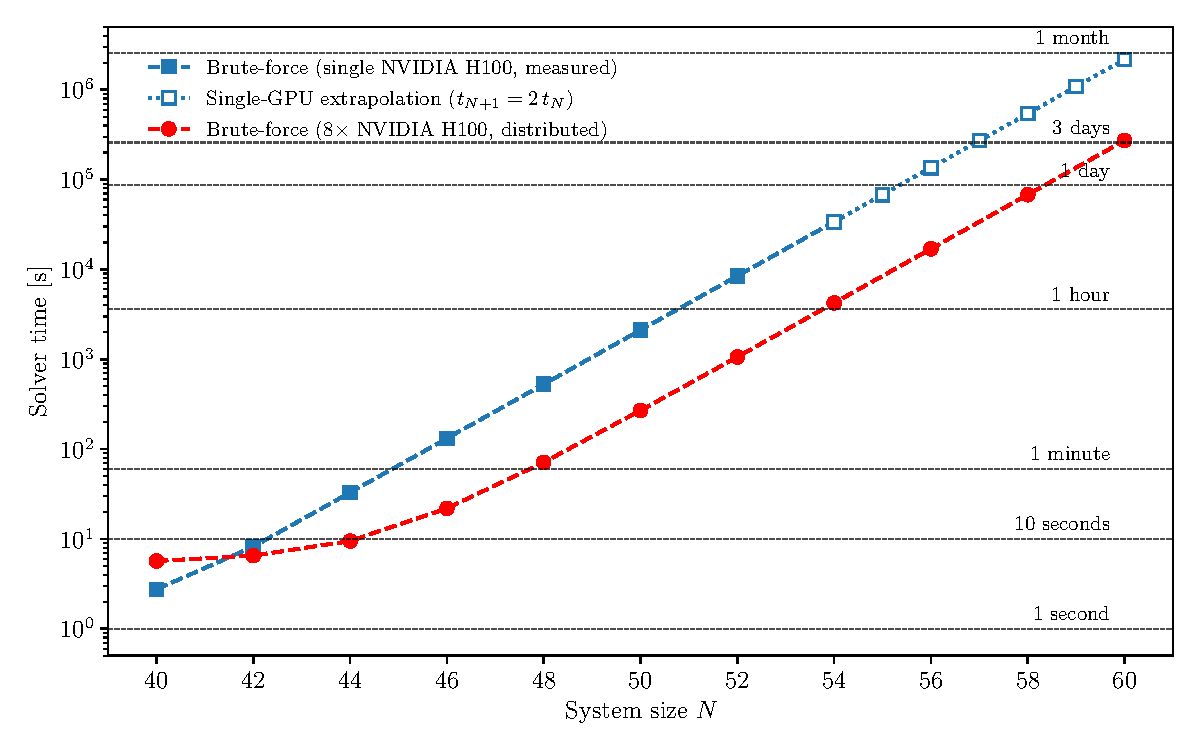
\includegraphics[width=0.95\textwidth]{distributed.pdf}
\caption{Wall-clock runtime of \texttt{omnisolver-bruteforce} on all-to-all
    random Ising instances with $J_{ij},h_i\sim \mathcal{U}[-1,1]$, measured
    on a local in-house cluster of $8\times$ NVIDIA H100 (96\,GB) GPUs (two
    nodes $\times$ 4 GPUs). Each filled marker is a single solver run on
    one fixed instance per system size $N$, where $N$ is the number of Ising
    spins, so that $2^{N}$ configurations are enumerated. Blue squares:
    single-GPU sampler (one of the H100s, measured for $N=40,\dots,54$). Open
    blue squares: doubling-rule extrapolation $t_{N+1}=2\,t_N$ from the largest
    measured single-GPU point to $N=60$. Red circles: distributed sampler
    on all eight GPUs with $k=3$ (measured for $N=40,\dots,60$). The two curves
    cross between $N=40$ and $N=42$; from $N=52$ onward the
    single-GPU-to-distributed runtime ratio settles at the linear-scaling value
    $\approx\!8$. Table~\ref{tab:efficiency} lists the corresponding speedups
    and parallel efficiencies.}
\label{fig:runtimes}
\end{figure}

\paragraph{Precision of the reported energies}
Because the GPU backend operates in \texttt{float32} on the fast ground-state
path, returned energies are subject to incremental-update roundoff. We therefore
re-evaluate the energy of every returned spin configuration from scratch in
\texttt{float64}. Across all twenty measured runs the roundoff of the
\texttt{float32} accumulator, obtained as the deviation between the reported and
the recomputed energy, stays below $1\times 10^{-5}$ in every run --- at most
$8.4\times 10^{-6}$, at $N=54$; at the largest size, $N=60$, it is
$6.4\times 10^{-6}$. Against energies of magnitude $\mathcal{O}(10^{2})$ this
amounts to about eight significant digits, consistent with the expected accuracy
of the stabilized \texttt{float32} accumulator. Three stored records ($N=46$,
$58$ and $60$) additionally contain a second, exactly known offset that is not
roundoff: the COO reader used at measurement time silently dropped the one
coupling of each of those instances whose magnitude lies below $10^{-4}$, so the
kernel enumerated a Hamiltonian differing from the one on disk by a single term
of up to $2.7\times 10^{-5}$. The returned configurations are unaffected --- they
match the optima of the full Hamiltonians, confirmed bit for bit by the
independent cross-check below --- and the roundoff figures above remove this
documented term; the reproduction package now parses the instance files exactly. The returned configuration is an exact bit string, and its energy can be
recomputed to \texttt{float64} accuracy by the caller at negligible cost, which is what we do
throughout. In every cross-check reported here the finite-precision deviation leaves the
selected state unchanged. Recomputing only that selected state cannot, however, prove that an
unretained, near-degenerate state was never misordered earlier in the floating-point search.
The benchmark results are therefore empirically cross-validated exhaustive-search minima; a
formal numerical certificate for arbitrary real coefficients would require exact or interval
arithmetic, or an error bound smaller than the gap to every competing state.

The two samplers also provide an independent check of the decomposition itself,
since at the eight sizes where both are feasible ($N=40,\dots,54$) they solve the
same instances by different routes: a single sweep over $2^{N}$ configurations on
one device, against eight independent sweeps over $2^{N-3}$ configurations each.
They return bit-identical configurations at all eight sizes, and their reported
energies differ by at most $8.2\times 10^{-6}$, i.e.\ at the level of the
\texttt{float32} roundoff quantified above. The fixed-variable split therefore
changes the wall-clock cost of the search, not its outcome.

\paragraph{Cost and effect of double precision}
Because the fast path is the single-precision one, it is fair to ask what the alternative
costs. Repeating the ground-state search at $N=40,\dots,46$ in both precisions on one H100
gives an unexpected answer. Excluding the $N=40$ warm-up outlier, \texttt{float64} is only
$2.0$--$2.3\%$ slower than \texttt{float32} (ratios of $1.02$ at
$N=42,44,46$), and both precisions return the same configuration at every size. The small timing difference suggests that the enumeration is not limited by floating-point
throughput but by the memory traffic and integer bookkeeping of the Gray-code sweep, so on
this hardware single precision buys working-set size rather than speed.

The compensated updates and the re-anchoring are enabled for \texttt{float32} only, so the
double-precision path runs unstabilized. In the measured range that is empirically
inconsequential: the \texttt{float64} accumulator stays within $10^{-13}$ of the from-scratch
recomputation at every size up to $N=46$, against $1$--$4\times 10^{-6}$ for stabilized
\texttt{float32}. (An earlier revision of this experiment showed an apparent \texttt{float64}
drift of $2.7\times 10^{-5}$ at $N=46$; it was exactly the dropped-coupling offset documented
above, not accumulation error.) Whether the unstabilized double-precision accumulator stays
clean at larger $N$ is unmeasured, which is why extending the stabilization to that path
remains listed as future work. The practical guidance is unchanged: use the default
\texttt{float32} path with its stabilization and, when a certified numerical value is wanted,
recompute the energy of the returned configuration in \texttt{float64} on the host, as done
throughout this paper.

\paragraph{Verification against a simulated-bifurcation solver}
Using the same recomputation we cross-check, on the identical instances, the heuristic whose
answers a certifying solver is meant to validate: a discrete simulated-bifurcation solver
(dSB), which we distribute with this article as \texttt{benchmarks/sbm.py}. It integrates all
replicas simultaneously, so one step is a single dense
$(N\!\times\!N)\,(N\!\times\!R)$ product and the whole run costs
$\mathcal{O}(N^{2}R\,\times\,\mathrm{steps})$ --- independently of the exponential cost of
\emph{certifying} the optimum, which is what makes a heuristic worth certifying in the first
place. We run it in \texttt{float64} with $R=2^{12}=4096$ parallel replicas, $3{,}000$
integration steps and seed 42. A probe selects one global time step from
$\{0.25,0.5,0.75,1.0,1.25\}$, and the coupling scale is
$c_0=0.5/(\sqrt{N}\,\mathrm{std}(J))$; we report the lowest-energy replica. At $N=60$ this
takes well under a minute on a CPU.

The heuristic is compared against every stored single-GPU and distributed result: twenty runs
over $N=38,\dots,60$, comprising all measured points of Fig.~\ref{fig:runtimes} plus one stored
distributed run at $N=38$, below the figure's range. On each of them the configuration it returns is bit-identical to the
certified ground state (Hamming distance $0$), and the energy of that configuration agrees
with the \texttt{float64} recomputation to $6\times 10^{-14}$. The Simulated Bifurcation
Machine therefore reaches the same exhaustive-search minimum on this instance family throughout the
measured range. The two solvers' \emph{reported} energies differ by at most
$2.5\times 10^{-5}$, and that residual is attributable entirely to the brute-force side: the
heuristic integrates and reports in \texttt{float64}, so its own energies sit
within $10^{-13}$ of the recomputation, while the exhaustive search reports from the
single-precision fast path --- including, at three sizes, the documented dropped-coupling
offset. The difference is bookkeeping on one side, not a
difference in the configurations found. This is precisely the
kind of statement that cannot be made without a certifying solver at hand, and it illustrates
the intended role of the plugin.

Shipping the heuristic alongside the article's reproduction package is deliberate: the comparison is only as
reproducible as its weaker half, so the verification needs neither GPU hardware nor an external
solver implementation; its ordinary Python and NumPy dependencies are declared. The solver, the driver that produces the verification tables
(\texttt{benchmarks/verify\_sbm.py}), the resulting tables themselves and all
\texttt{benchmarks/instances/*.txt}, \texttt{benchmarks/results/single-gpu/*.json} and
\texttt{benchmarks/results/distributed/*.json} files behind Fig.~\ref{fig:runtimes} and
Table~\ref{tab:efficiency} are distributed with the article
repository \href{\datarepo}{\datareponame}.

\paragraph{Instance families and targeted multi-solver comparison}
The present plugin performs complete enumeration, evaluating all $2^{N}$ assignments
regardless of the coefficient distribution. Its own runtime is therefore essentially
independent of instance family, apart from negligible best-state bookkeeping. This property is
specific to this implementation: branch-and-bound and structure-aware exact methods can prune
the search and may have strongly family-dependent behavior.

We evaluate the plugin in its intended role as a certification backend using two
algorithmically distinct heuristics on the same twenty $N=44$ instances: five each with
couplings uniform on $[-1,1]$, bimodal $J_{ij}\in\{-1,+1\}$, Gaussian, and sparse at $20\%$
density. The dSB solver uses $4096$ replicas, $3000$ integration steps, seed 42,
\texttt{float64} dynamics and its automatically tuned time step. The simulated-annealing (SA)
solver~\cite{kirkpatrick1983optimization} is
\texttt{dwave.samplers.SimulatedAnnealingSampler}; it uses $4096$ reads, $3000$ sweeps, a
geometric inverse-temperature schedule, randomized spin-update order and deterministic seeds
$420000,\dots,420019$. These are documented method-specific budgets: a dSB integration step
and an SA sweep are not treated as equal units of work.

Both heuristics reach a certified optimum on all twenty instances. The dSB state is identical
to the stored certified state on seventeen instances and the SA state on sixteen; every
different state occurs in the bimodal family and has the same integer energy, reflecting
ground-state degeneracy rather than an optimization error. Independent \texttt{float64}
evaluation puts each selected state's energy within $3.2\times10^{-13}$ of the certified value.
The family-level results are shown in Table~\ref{tab:multisolver}; both heuristics were rerun
sequentially by the same driver on the same CPU host (\texttt{alice}, an H100-equipped server),
while their timings describe method-specific budgets rather than equal work.

\begin{table}[H]
\centering
\small
\begin{tabular}{|l|cc|rr|}
\hline
 & \multicolumn{2}{c|}{certified optima} & \multicolumn{2}{c|}{median time [s]} \\
family & dSB & SA & dSB & SA \\
\hline
uniform  & $5/5$ & $5/5$ & 10.02 & 10.30 \\
bimodal  & $5/5$ & $5/5$ &  9.44 & 16.60 \\
Gaussian & $5/5$ & $5/5$ &  9.24 &  9.38 \\
sparse   & $5/5$ & $5/5$ &  8.79 & 11.37 \\
\hline
all      & $20/20$ & $20/20$ &  9.21 & 10.80 \\
\hline
\end{tabular}
\caption{Targeted comparison of two heuristic mechanisms against exhaustive-search
certificates on the same twenty $N=44$ instances. Times are wall-clock medians under the
method-specific budgets stated in the text, not equal-work comparisons. Each selected-state
energy is recomputed independently in \texttt{float64}; complete per-instance states,
seeds, timings, gaps and instance hashes are stored in
\protect\path{benchmarks/results/multi_solver/run_20260816_125511.json}.}
\label{tab:multisolver}
\end{table}

\paragraph{A planted family where certification is decisive}
The four families above show the heuristics succeeding; they do not show why a certifying
backend is needed. The complement is the Wishart planted ensemble~\cite{hamze2020wishart}, a
fully connected zero-field family with tunable ruggedness: a planted state $t$ is drawn, $M
\approx \alpha N$ Gaussian columns are projected orthogonal to it and collected in $W$, and
the couplings are $J_{ij}=(WW^{\mathsf{T}})_{ij}/N$. The construction makes the ground-state
energy known analytically, $E_0=-\mathrm{tr}(WW^{\mathsf{T}})/(2N)$, attained exactly by
$\pm t$, and the ratio $\alpha=M/N$ tunes the depth of the first-order barrier in the energy
landscape; small $\alpha$ is the rugged regime. On twenty instances per
$\alpha\in\{0.20,0.25,\dots,0.50\}$ at $N=40$, the dSB solver under the same budgets as above
undergoes a sharp transition (Fig.~\ref{fig:wishart}): it recovers the certified optimum on
every instance at $\alpha\geq0.45$ and on $18/20$ at $\alpha=0.4$, but on only $3/20$, $1/20$
and $0/20$ at $\alpha=0.3$, $0.25$ and $0.2$, terminating $0.14$--$1.8\%$ above the optimum
--- on wrong, near-optimal configurations that nothing short of a certified reference exposes.
The brute-force sampler certifies each instance in $\approx\!2$\,s on one H100, at this size
less than a single $7$--$9$\,s dSB run; it returns the planted configuration on all $140$
instances, and its \texttt{float64}-recomputed certificate matches the analytic $E_0$ to
$4\times10^{-15}$ on every one, which checks the whole pipeline, from the instance files to
the kernel, against a value independent of both solvers. The deterministic generator, the instances and the raw records ship with the
article, and the heuristic side of the comparison is re-checkable without a GPU against the
analytic optimum (Sec.~\ref{sec:reproduction}).

\begin{figure}[t]
\centering

\includegraphics[width=0.85\textwidth]{wishart.pdf}
\caption{Fraction of Wishart planted instances on which a single run of the shipped dSB
    heuristic, under the budgets of Table~\ref{tab:multisolver}, reaches the certified
    optimum, as a function of the ruggedness parameter $\alpha=M/N$ at $N=40$. Twenty
    instances per $\alpha$, one run each; error bars are $95\%$ Wilson intervals for the
    per-instance success probability, and each point is annotated with its count.
    Exhaustive certification costs $\approx\!2$\,s per instance throughout, and every
    certificate matches the analytic $E_0$ of its instance.}
\label{fig:wishart}
\end{figure}

\paragraph{QUBO path and exact-solver checks}
The QUBO and Ising interfaces use the same computational path: both samplers convert a SPIN
model to its BINARY equivalent, solve it as a QUBO and convert the result back, so the reported
timings are QUBO timings. The only Ising-specific cost is an $O(N^{2})$ host-side
transformation outside the measured region. Loading the same coefficient files once with each
variable type confirms this: over $N=42,\dots,50$ the ratio of BINARY to SPIN wall-clock time
is $0.998$--$1.000$. Correctness is cross-checked against \texttt{dimod.ExactSolver} on
instances small enough for CPU enumeration and by independent \texttt{float64} recomputation
at benchmark scale. These checks validate implementation correctness; they are not a claim of
comparative performance against every exact algorithm.

\paragraph{Limitations and intended scope}
Exhaustive enumeration scales as $O(2^N)$ irrespective of GPU count or
numerical precision: the update lowers the constant factor and removes a
\texttt{float32} drift pitfall, but it cannot change the underlying
complexity. The plugin is therefore intended as a \emph{verification and
certification backend} for QUBO/Ising research pipelines---providing
ground-truth optima against which heuristics, annealers, and NISQ-era
quantum approaches can be calibrated---rather than as a routine optimizer
for application-scale problems, where heuristic solvers such as the SBM
remain the appropriate primary tool. The concrete hard limits of the current
implementation are: (i) the per-worker spin configuration is held in a 64-bit
word, so each subproblem is limited to $N-k \leq 64$ unfixed variables; with
$k=\texttt{num\_fixed\_vars}$ fixed variables the distributed sampler therefore
supports $N \leq 64+k$, while the single-GPU sampler is capped at $N \leq 64$,
and both samplers validate the applicable bound before launching; (ii) the
per-worker \texttt{suffix\_size} (the number of
variables forming the resident enumeration chunk) is bounded by the GPU's
L2/working-set budget and was set to $23$ on the H100 (96\,GB) in our runs, so
larger $N$ is handled by sweeping more fixed-size chunks; raising
\texttt{num\_fixed\_vars} is needed to distribute that work or to maintain
$N-k\leq64$, rather than to enlarge \texttt{suffix\_size}; (iii) the numerical stabilization applies to the
\texttt{float32} ground-state path and is enabled when the size seen by the
kernel is at least $40$ variables, that is for $N-k \geq 40$ in distributed
runs, so the two smallest distributed points of Fig.~\ref{fig:runtimes} were
obtained on the unstabilized path---they nevertheless agree bit-for-bit with the
stabilized single-GPU runs at the same sizes; (iv) the projected runtimes
for $N > 60$ are back-of-the-envelope extrapolations under the empirical
$t_{N+1}=2\,t_N$ rule and may drift by a small constant factor on different
stacks; and (v) the scaling measurements span two nodes and eight GPUs, which is
the extent of the hardware available to us. Within that envelope both strong and
weak scaling are measured on every tested power-of-two GPU count and realizable node layout
(Table~\ref{tab:scaling}), and the controller is measured directly up to $2^{16}$
subproblems (Table~\ref{tab:controller}), but the behavior of the \emph{search}
phase beyond eight devices, and with more than one node boundary, remains an
extrapolation. Reported runtimes
additionally depend on the hardware and software stack (GPU model, CUDA
toolkit, Ray version, interconnect), so the absolute timings in
Fig.~\ref{fig:runtimes} should be read as a hardware-specific operating
point rather than a universal guarantee.

\section{Illustrative example}
\label{sec:example}
The plugin is distributed as \texttt{omnisolver-bruteforce} on PyPI
(\texttt{pip install omnisolver-bruteforce}) and is usable either
stand-alone or through the Omnisolver CLI, under which it registers as the
\texttt{bruteforce-gpu} solver; the distributed sampler additionally requires
\texttt{ray} to be present in the environment. Since the distribution is a
source archive, installation compiles the CUDA extension locally and therefore
needs a CUDA Toolkit installation. The sources and the documentation of the
plugin are in the
\href{https://github.com/euro-hpc-pl/omnisolver-bruteforce}{plugin
repository}~(C2). The benchmark and plotting scripts used to produce
Fig.~\ref{fig:runtimes} and Table~\ref{tab:efficiency} are in the article
repository \href{\datarepo}{\datareponame} under \texttt{benchmarks/}, together
with the instances, the raw results and the verification tables they consume, so
that the figure and the table can be regenerated from a single checkout. The same
directory contains the drivers of the scaling, precision, QUBO and instance-family
experiments reported above, and a NumPy implementation of the
simulated-bifurcation heuristic used for the verification. The separate SA cross-check uses
the pinned \texttt{dwave-samplers} dependency listed in
\texttt{benchmarks/environment.yml}.
Sec.~\ref{sec:reproduction} is a guide to that directory.

A minimal distributed-sampler invocation looks as follows:

\begin{lstlisting}[language=Python,caption={Minimal distributed brute-force example},label={lst:bf-min}]
from omnisolver.bruteforce.gpu.distributed import DistributedBruteforceGPUSampler
from dimod.serialization import coo

with open("instance.txt") as fd:
    bqm = coo.load(fd, vartype="SPIN")

sampler = DistributedBruteforceGPUSampler()
result = sampler.sample(
    bqm,
    num_states=1,
    num_fixed_vars=3,
    suffix_size=23,
    grid_size=8192,
    block_size=1024,
    partial_diff_buffer_depth=10,
    num_steps_per_kernel=8192,
)
print(result.first.energy, result.info["solve_time_in_seconds"])
\end{lstlisting}

For multi-GPU execution, Ray must be started on the head and worker
nodes (here, an 8-GPU two-node setup with 4 GPUs per node), after which the
benchmark script reproduces the curve in Fig.~\ref{fig:runtimes}:

\begin{lstlisting}[language=bash,caption={Ray startup and benchmark command used to produce Fig.~\ref{fig:runtimes}},label={lst:ray-commands}]
# Head node
ray stop --force
ray start --head --port=6379 --num-gpus=4

# Worker node
ray stop --force
ray start --address='<HEAD_NODE_IP>:6379' --num-gpus=4

# Run benchmark sweep (from the article repository root)
python benchmarks/bf.py --start 40 --stop 60 --step 2 \
                        --sampler-mode distributed \
                        --skip-existing
\end{lstlisting}

\section{Reproducing the reported results}
\label{sec:reproduction}
Every number in this paper is produced by code and data in the
\texttt{benchmarks/} directory of the article repository
\href{\datarepo}{\datareponame}, and a substantial part of it can be re-checked
\emph{without a GPU at all}. This section is a guide to that directory.

\paragraph{What is where}
\texttt{benchmarks/} holds the instances (\texttt{instances/}), the raw
per-run results (\texttt{results/}, one subdirectory per experiment), the
verification tables (\texttt{bf\_sbm\_verification\_*.csv}), the solver
drivers \texttt{bf.py} and \texttt{plot\_distributed.py} that produce
Fig.~\ref{fig:runtimes}, one driver per experiment
(\texttt{exp\_*.py}), the NumPy simulated-bifurcation solver \texttt{sbm.py}
with its verification driver \texttt{verify\_sbm.py}, the simulated-annealing
comparison driver \texttt{exp\_multi\_solver.py}, the planted-Wishart generator
\texttt{gen\_wishart.py}, and the launchers in
\texttt{scripts/}. Shared helpers live in \texttt{bench\_common.py}: the
environment descriptors recorded by the revision experiments, the detection of the Ray
topology, and a per-size instance generator whose output does not depend on
which other sizes are generated alongside it. The long-running scaling launchers
skip completed points, while the E7 and E8 evidence drivers create non-overwriting
outputs unless replacement is requested explicitly.

\paragraph{Prerequisites}
A CUDA-capable environment with the plugin installed, as in
Sec.~\ref{sec:example}, on \emph{every} node that will run subproblems: Ray
ships no code, so a worker without the package cannot solve one. The
multi-node launchers additionally need password-less \texttt{ssh} from the head
node to the workers. The script \texttt{scripts/preflight.sh} checks all of
this---environment activation, imports, visible devices---and prints the CUDA
toolkit, driver and package versions of each node side by side, so that a
mismatch between them is found before, rather than after, a long run.
The supplied Conda environment also installs \texttt{dwave-samplers} for the CPU-only E8
comparison and the Python plotting dependencies; rendering Fig.~1 additionally requires a
system \LaTeX{} installation because the plot uses Matplotlib's \texttt{text.usetex} mode.

\paragraph{The reproduction path}
Table~\ref{tab:reproduction} lists one launcher per claim. The whole set is run
by \texttt{scripts/run\_all.sh}, which executes the CPU-only diagnostics first and then the
GPU experiments, records
each result under \texttt{results/}, keeps a timestamped log, and continues past
a failing stage rather than aborting the batch. The verification, multi-solver
and controller-cost entries need no GPU. Long-running launchers resume at completed points,
and E6--E8 create timestamped, non-overwriting evidence records. The short E3--E5 drivers and
the verification driver update their documented canonical outputs, so those files should be
copied before an intentional repeat if both runs are to be retained.

\begin{table}[H]
\setlength{\tabcolsep}{4pt}
\centering
\begin{tabular}{|p{4.2cm}|p{5.3cm}|p{2.0cm}|}
\hline
\textbf{Launcher} & \textbf{What it establishes} & \textbf{Cost} \\
\hline
\texttt{preflight} & both nodes can run the experiments; per-node toolchain
report & seconds, any \\
\hline
\texttt{verification} & every stored optimum re-checked in \texttt{float64} and
against dSB & 10\,min, CPU \\
\hline
\texttt{e8\_multi\_solver} & dSB and SA rerun on the same host against the same twenty certified
$N=44$ instances (Table~\ref{tab:multisolver}) & 8\,min, CPU \\
\hline
\texttt{e3\_controller\_cost} & local controller cost up to $2^{16}$ subproblems
(Table~\ref{tab:controller}) & 30\,min, CPU \\
\hline
\texttt{e7\_boundary\_cost} & matched end-to-end task returns under local, remote and mixed
placement across one node boundary & 5\,min, 2 nodes \\
\hline
\texttt{e6\_instance\_families} & dSB against certified optima over four
coupling families & 18\,min, 1 GPU \\
\hline
\texttt{e9\_wishart} & dSB against certified and analytic optima on the rugged
Wishart family (Fig.~\ref{fig:wishart}) & 40\,min, 1 GPU \\
\hline
\texttt{e4\_precision} & \texttt{float32} against \texttt{float64} on the
ground-state path & 6\,min, 1 GPU \\
\hline
\texttt{e5\_qubo} & QUBO and Ising runtimes on identical coefficients &
1.6\,h, 1 GPU \\
\hline
\texttt{e1\_strong\_scaling} & speedup and parallel efficiency over GPU count
and node layout & 2\,h, 1--8 GPUs \\
\hline
\texttt{e2\_weak\_scaling} & weak scaling at constant work per GPU &
4\,h, 1--8 GPUs \\
\hline
\texttt{manuscript\_figure} & Fig.~\ref{fig:runtimes} and
Table~\ref{tab:efficiency} & see caption \\
\hline
\end{tabular}
\caption{Launchers provided for reproducing the reported results, in the order in
which \texttt{scripts/run\_all.sh} executes them; each is the script
\texttt{scripts/run\_<name>.sh}, except \texttt{preflight}. Costs are for
H100-class GPUs, measured on the runs reported in this paper, and are dominated by the
exhaustive searches themselves; the whole set without the figure is an overnight job. \texttt{manuscript\_figure}
re-draws the figure in seconds when the published results are present, since it
skips sizes that already have a result file; regenerating them from scratch is
the only multi-day item, because $N=58$ alone takes $\approx\!19$\,h and $N=60$
$\approx\!3.15$ days.}
\label{tab:reproduction}
\end{table}

\paragraph{Cluster topologies}
Ray cannot rearrange a running cluster, so the GPU layout is fixed when Ray is
started on each node. \texttt{scripts/ray\_cluster.sh} does that for a requested
layout, written \texttt{<nodes>x<GPUs per node>}, and the experiment drivers
then \emph{detect} the layout, refuse to run if it differs from the one
requested on the command line, and record it with the result---so a run cannot
be silently mislabeled:

\begin{lstlisting}[language=bash,caption={Driving the cluster by hand; the experiment launchers do this internally},label={lst:topology}]
./benchmarks/scripts/ray_cluster.sh start 2x1   # 1 GPU on each of two nodes
./benchmarks/scripts/ray_cluster.sh status      # detected topology, as JSON
./benchmarks/scripts/ray_cluster.sh stop
\end{lstlisting}

Fewer GPUs per node than the machine has are obtained by masking
\texttt{CUDA\_VISIBLE\_DEVICES} before starting Ray. This is what makes the pairs
\texttt{1x2}/\texttt{2x1} and \texttt{1x4}/\texttt{2x2} directly comparable: the
same number of GPUs, differing only in whether a node boundary is crossed. On a
two-node cluster that difference is the closest available measure of the
multi-node behavior of the decomposition.

\paragraph{Verification without a GPU}
The verification of Sec.~\ref{sec:description} can be repeated on a laptop.
\texttt{sbm.py} integrates all replicas of the discrete simulated-bifurcation
dynamics simultaneously, so one step is a single dense
$(N\!\times\!N)(N\!\times\!R)$ product and the cost is
$\mathcal{O}(N^{2}R\,\times\,\mathrm{steps})$, independent of the exponential cost
of certifying the optimum; $N=60$ with $R=4096$ replicas and $3{,}000$ steps
takes well under a minute. Running

\begin{lstlisting}[language=bash,caption={Re-checking every certified optimum without a GPU},label={lst:verify}]
python benchmarks/verify_sbm.py --check
\end{lstlisting}

recomputes the energy of every stored brute-force configuration from scratch in
\texttt{float64}, runs the heuristic on the same instance, writes the
\texttt{bf\_sbm\_verification\_*} tables and reports, for every instance, whether
the heuristic reached the certified optimum and at what Hamming distance.
The targeted multi-solver comparison is likewise CPU-only:

\begin{lstlisting}[language=bash,caption={Re-running dSB and simulated annealing on the twenty certified family instances},label={lst:multisolver}]
./benchmarks/scripts/run_e8_multi_solver.sh
\end{lstlisting}

It validates the immutable E6 certificate, records every instance hash and checks that each
file remains unchanged during the run, reruns both heuristics on the same host, then records
both configurations, deterministic seeds, selected states,
independently recomputed selected-state energies and the family summaries used in
Table~\ref{tab:multisolver}.

\section{Conclusions and outlook}
\label{sec:conclusions}
This update turns the exhaustive-search plugin announced
in~\cite{jalowiecki2021omnisolver}, whose CUDA core originates
in~\cite{jalowiecki2021brute}, into a released and API-stable certification
backend: it ships a versioned distributed sampler that executes the
fixed-variable decomposition across multiple GPUs and hosts through Ray,
resolves the \texttt{float32} stability issue of the fast ground-state path, and
hardens the enumeration bookkeeping for large configuration sizes---all without
changing the public sampler API. On dense random Ising instances we now certify
exhaustive ground states up to $N=60$ on $8\times$ H100 GPUs, empirically
confirming the asymptotic $t_{N+1}=2\,t_N$ doubling regime from $N=52$, and we
quantify the strong scaling of the decomposition, which reaches $93\%$ parallel
efficiency at $N=48$ and the ideal $8\times$ speedup from $N=52$ on. On a planted
rugged family the certified optima expose heuristic near-misses of up to $1.8\%$
at a size certified in seconds --- the concrete regime such a backend
exists for. Natural
next steps are: (i) reducing the per-task scheduling overhead that
Table~\ref{tab:controller} identifies as one measured source of scaling overhead, for
instance by grouping several fixed assignments into one task so that the number of
Ray tasks grows more slowly than $2^{k}$;
(ii) extending the scaling study beyond one node boundary, which is the one
question our two-node cluster cannot settle: a single boundary changes the reported solve-phase
wall-clock time by less than we can resolve; $1.5\%$ is the empirical repeatability scale of the
two-node timings, not a statistical upper bound. The separate task-return diagnostic does resolve a payload-dependent return
cost, but cannot establish how it compounds or saturates over many boundaries; (iii) exposing the re-anchoring
cadence and the compensated-update mode as user-tunable knobs for instance families
where the default policy is suboptimal, and extending the stabilization to the
double-precision path, which the measurements above show to be both affordable and
currently unstabilized; and (iv) archiving the reproduction directory of
Sec.~\ref{sec:reproduction} under a persistent identifier, so that the fixed
seeds, the recorded hardware and toolkit descriptors and the command presets it
already contains remain citable independently of the repository hosting them.

\section*{Declaration of competing interest}
The authors declare that they have no known competing financial interests or
personal relationships that could have appeared to influence the work reported
in this paper.

\section*{Acknowledgments}
This work was supported by the National Science Center (NCN), Poland, via
project Sonata Bis 10, No.~2020/38/E/ST3/00269 (B.G.) and Sonata Bis 15,
No.~2025/58/E/ST6/00422 ({\L}.P.). Quantumz.io Sp.~z~o.o.\ acknowledges
support received from the Polish Agency for Enterprise Development (PARP),
Poland, under Project No.~FENG.01.01-IP.02-0625/23, titled
\textit{Dynamic allocation of resources in industrial ecosystems susceptible
to disturbances using physics-inspired algorithms and machine learning}.

\bibliographystyle{elsarticle-num}
\bibliography{bruteforce.bib}

\end{document}
